
In this section the main concept of how the controlling in \GLS{eeros} is working and how it may be optimized or improved.

\section[Overview]{Overview} \label{sec:concept-overview}

As base system, \GLS{ros} is taken into account.
With \GLS{ros}, the whole communication between different parts (nodes) of a system, can be handled quite easily.
For this, \GLS{ros} provides topics and services, where nodes can publish and consume messages or subscribe to and provide services.
Every node can publish or receive messages in all topics, but also request or provide information from/as services.
Topics are the main communication interface of providing information between the nodes in real-time, whereas services are more an asynchronous way of requesting information.
For example the topic \textit{/joint\_states} is used to publish the state of all joints of a robot.
A Service on the other hand can be used to request the temperature from a battery, which is not really important for maneuver a robot but may be interesting for future calculations.

\begin{figure}[H]
    \centering
    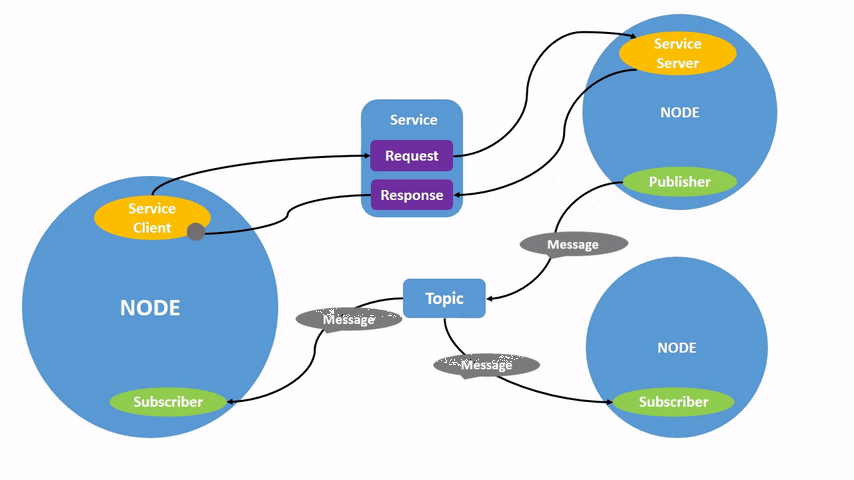
\includegraphics[width=0.6\linewidth]{images/NodesTopicandService}
    \caption[\GLS{ros} Nodes, Topics and Services]{Visualization\protect\footnotemark of \GLS{ros} \Glspl{node}, \Glspl{topic} and Services. Each Node can provide and offer topics and services but can also consume them.}
    \label{fig:ros-nodes-topics-services}
\end{figure}

\footnotetext{\url{http://docs.ros.org/en/humble/Tutorials/Beginner-CLI-Tools/Understanding-ROS2-Nodes/Understanding-ROS2-Nodes.html}}


\subsection[Gazebo]{Gazebo as a Node} \label{sec:gazebo-node}

\Gls{gazebo} is a physics simulation which works quite well with \GLS{ros}.
To communicate with \GLS{ros} there are plugins substantial:

\begin{description}
    \item[ibgazebo\_ros\_joint\_state\_publisher] is publishing all joint states to the \GLS{ros}-\Gls{topic} \textit{/joint\_states}.
    \item[libgazebo\_ros\_diff\_drive] can be used to consume messages from a topic (normally \textit{/cmd\_vel}) and apply them to wheels from a robot. The consumed message is a \textit{Twist}, which expresses velocity in free space broken into its linear and angular parts.
    \item[libgazebo\_ros\_joint\_pose\_trajectory] can be used to consume messages from a topic (normally \textit{/set\_joint\_trajectory}) and apply them to a joints. The message is a \textit{JointTrajectory} which defines the trajectory for each joint.
\end{description}

There are third-party ones which could be used for example as a motor driver.
Sadly that one is built on top of \GLS{ros}-1 and is not (yet?) ported yet to \GLS{ros}-2.


\subsection[EEROS]{EEROS as a Node} \label{sec:eeros-node}

\GLS{eeros} can be used as a layer between \GLS{ros} and the Hardware as an easy to use Framework for controlling, measuring and communication.\footnote{This is how I understood \GLS{eeros} and what it is for.}
\GLS{eeros} is built based on Blocks, which can be assembled individually based on their functionality.
Each Block is processed regularly, initiated by a central executor, and can react to events and actions.
The Hardware is separated through a \GLS{hal} what should make it easy to replace the Hardware by a different technology or even a simulation.


\subsubsection[EEROS Executor]{The EEROS Executor} \label{sec:eeros-executor}

The heart of each \GLS{eeros} Node is the Executor.
All Blocks are registered through a safety-system and are processed regularly.

The Executor has mainly the following different modes it can run in:

\begin{itemize}
    \item[\textbf{Normal}] All Messages from a \Gls{topic} are received and stored in a queue. As soon as \GLS{eeros} decides to process the blocks, all (or only the newest) messages are processed.
    \item[\textbf{Sync}] \GLS{eeros} is synchronized with a Subscriber-Topic. The Blocks are processed on every incoming message.
    \item[\textbf{EtherCAT}] \GLS{eeros} is synchronized with an \Gls{ether} stack and will process the blocks as soon as a signal from \Gls{ether} is received. All Messages from any subscribed \gls{topic} are stored in a queue until then.
\end{itemize}

\begin{figure}[H]
    \centering
    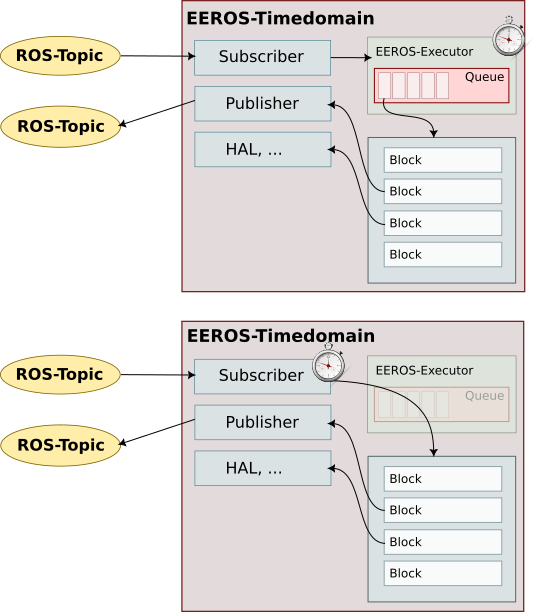
\includegraphics[width=0.6\linewidth]{images/eeros-executor}
    \caption[\GLS{eeros} Overview]{Visualization of \GLS{eeros}-Executor and the two different modes it will process the Blocks. The upper one shows the three modes where \GLS{eeros} is the in charge, the lower one where a subscription to a topic is in charge and processes each received message directly.}
    \label{fig:eeros-overview}
\end{figure}


\subsection[Simulation time]{Simulation Time} \label{sec:simulation-time}

As already shown in \ref{sec:eeros-executor}, \GLS{eeros} can be synchronized with different peripheral systems.
Depending on which mode is used, \GLS{eeros} runs with different simulation times:

\begin{itemize}
    \item[\textbf{System}] \GLS{eeros} is normally the main clock and uses the system time for processing.
    \item[\textbf{ROS-Time}] \GLS{eeros} will use the ROS-Time for the timing.
    \item[\textbf{EtherCAT}] A connected \Gls{ether}-Device defines the timing.
    Actually the time between messages from \Gls{ether} defines the timing.
    \item[\textbf{Topic}] A \GLS{ros}-\Gls{topic} can be used in combination with a Subscriber.
    This \gls{topic} has to be managed by an other node, for example \Gls{gazebo}.
\end{itemize}



\subsubsection[Mistakes]{Common Mistakes with Topics} \label{sec:ros-common-mistakes}

A common tar-pit when working with \GLS{ros}-\Glspl{topic}\footnote{As a software and security engineer my understanding of \GLS{ros} was more like a Low-Level Message-Queue like MQTT for IoT devices, RabbitMQ or any other MQ.} is a subscription to \gls{topic}-A and a publisher to the same \gls{topic}.
In such a setup, the subscriber will immediately receive the new message sent from the publisher, notify the publisher which is sending out a message again.
This will \gls{dos} the whole system.

A Message from a \GLS{ros}-\Gls{topic} has a header with the time it was sent.
A message has no information about from which \Gls{node} it is coming from.
Therefore a node cannot separate messages and should never publish to the same topics it is subscribed to.



